\section{Communication}
\label{sec:communication}

\subsection{Message construction}
\label{sec:msg}
The goal of communication is to increase the knowledge base of agents and to improve coordination among them. However, in a disaster scenario, communication can be unreliable and bandwidth is limited. To address these problems, our communication strategy is based on a simple protocol. We define three message types for each kind of problem (blockades, burning buildings and buried civilians) the agents may encounter:

\begin{itemize}
 \item \msg{Report}: the agent found a problem and reports it along with relevant information to its teammates. % Report messages contain information about the problem so that other agents can update their knowledge bases and reason about the recently discovered problem, that is, deciding to engage or not.

 \item \msg{Engaging}: the agent decided to engage in a problem. \msg{Engaging} messages also contain information about the problem so that other agents can update their knowledge bases even if the problem was reported earlier.

 \item \msg{Solved}: the agent solved the problem and no further action about it is required. %Solved messages do not contain information about the problem status (such as the temperature of a building) since the problem was solved and no further action is needed.
\end{itemize}

%Coordination among agents, i.e., requesting help for more effort-demanding tasks require a special protocol, described in Section \ref{sec:recruiting}.

%In order to save radio bandwidth and maximize the amount of data shared between agents, our communication will use a data compression algorithm. Each agent is responsible for compressing/decompressing the communication data.

\subsection{Recruiting protocol}
\label{sec:recruiting}
When an agent estimates that it needs help to perform a task, it starts a recruitment process that consists of the following three steps: first, a \msg{request} message is sent by the recruiter agent to other agents. Agents who receive the \msg{request} message and are available to help  send back a \msg{committed} message. 
Receiving \msg{committed} messages allows the recruiter agent to select the teammates that will help best in the task. 
The recruiter sends \msg{engage} messages to selected teammates and \msg{release} to non-selected ones.  Note that \msg{engage} messages used in the recruitment protocol are different from \msg{engaging} messages used in general communication (Section \ref{sec:msg}). This recruitment process is based on the recruitment protocol of eXtreme-Ants \cite{Santos&Bazzan2009optmas}, which is a scalable task allocation algorithm based on swarm intelligence. Figure \ref{fig:auction} illustrates the recruitment process.

\begin{figure}[ht]
  \centering
  \subfigure[]{
    {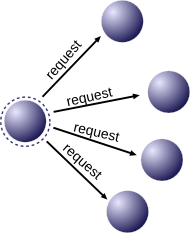
\includegraphics[width=2.4cm]{img/request.png}}
    \label{fig:request}
  }%
  \subfigure[]{
    {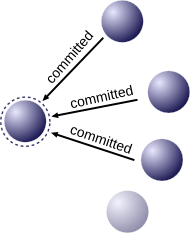
\includegraphics[width=2.4cm]{img/offer.png}}
    \label{fig:offer}
  }%
  \subfigure[]{
    {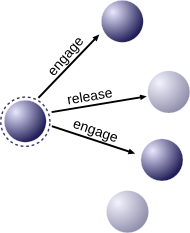
\includegraphics[width=2.4cm]{img/commit.png}}
    \label{fig:commit}
  }%

  \caption{Recruitment process: \subref{fig:request} recruiter (circled with dashed line) sends \msg{request} messages; \subref{fig:offer} agents who decide to help respond with \msg{committed} messages; \subref{fig:commit} recruiter sends \msg{engage} to selected teammates and dismisses non-selected ones with \msg{release} messages.}

 \label{fig:auction}
\end{figure}

%It should be noted that messages are always broadcasted in a given channel, that is, all agents can hear all messages in the channel. When it is said that a message is directed to a specific agent, the meaning is that the message is broadcasted in the channel but it has additional information so that non-targets of the message can ignore it.

% Sera implementado um leilão em 3 etapas (anúncio, recebimento de 'ofertas' e recrutamento) para bombeiros pedirem auxílio em tarefas dificeis.
% Compactação
